\documentclass[aps,prd,twocolumn,superscriptaddress,amsfont,amssymb,amsmath,nofootinbib,showpacs,balancelastpage]{revtex4-1}
%\documentclass[prd,superscriptaddress,twocolumn,floatfix]{revtex4}

\usepackage{graphicx,longtable,natbib,mathrsfs,color}
\usepackage{txfonts}

\newcommand{\bs}{\boldsymbol}
\newcommand{\diff}{{\mathrm d}}
\newcommand{\Cov}{\mathsf{C}}
\newcommand{\Fish}{\mathsf{F}}
\newcommand{\Cl}{\mathcal {C}}
\newcommand{\R}{\mathcal{R}}
\newcommand{\T}{\mathcal{T}}
\newcommand{\Msun}{M_\odot}

%
\def\apjl{Astrophys. J. Lett.}
\def\apjs{Astrophys. J. Suppl. Ser.}
\def\aj{Astron. J.}
\def\mnras{Mon. Not. R. Astron. Soc.}
\def\aap{Astron. Astrophys.}                % Astronomy and Astrophysics
\def\jcap{J. Cosmology Astropart. Phys.}
\def\aapr{Astron. Astrophys. Rev.}

\begin{document}

\addtolength{\hoffset}{-0.525cm}
\addtolength{\textwidth}{1.05cm}
\title{Displacement field paper}

%\author{Hao-Ran~Yu} \affiliation{}\email{haoran@cita.utoronto.ca}
%\author{Qiaoyin~Pan}
%\author{Ue-Li~Pen} \affiliation{}
%\author{Tong-Jie~Zhang} \affiliation{}
%---


%\date{Received \today; published -- 00, 0000}

\begin{abstract}
In this paper, we discover the ability of using displacement field to reconstruct initial linear perturbations in the early universe.
\end{abstract}

%\pacs{98.80.Es 95.36.+x}

\maketitle

\section{Introduction}\label{sec.intro}
Introduction goes here. Citation example \cite{2013MNRAS.436..540H}.
Cite Hong-Ming's 1D paper.

The rest of this paper is structured as follows. In section \ref{sec.method} we describe the simulation and reconstruction algorithm. In section \ref{sec.results} we show the results of the reconstruction. Discussion and conclusion are in \ref{sec.discussion}.



\section{Method}\label{sec.method}
Method goes there.

\subsection{Simulation}
Cosmological parameters, simulation parameters.

Initial conditions, get linear density field $\delta_L$. Run simulation by code {\tt CUBE} and get the nonlinear density field $\delta$ at $z=0$. {\tt CUBE} uses particle-ID (PID) to record the initial location of particles, and the information is tracked until the $z=0$ and we can get the displacement vector ${\bs s}\equiv{\bs x}-{\bs q}$ for every particle. Then these vectors are interpolated onto the initial Lagrangian coordinates ${\bs q}$ of particles and we get the displacement field ${\bs s}({\bs q})$.

\subsection{Reconstruction}
Get the raw reconstructed density field $\delta_R=-\nabla\cdot{\bs s}({\bs q})$.


%\begin{figure}[t] \centering
%  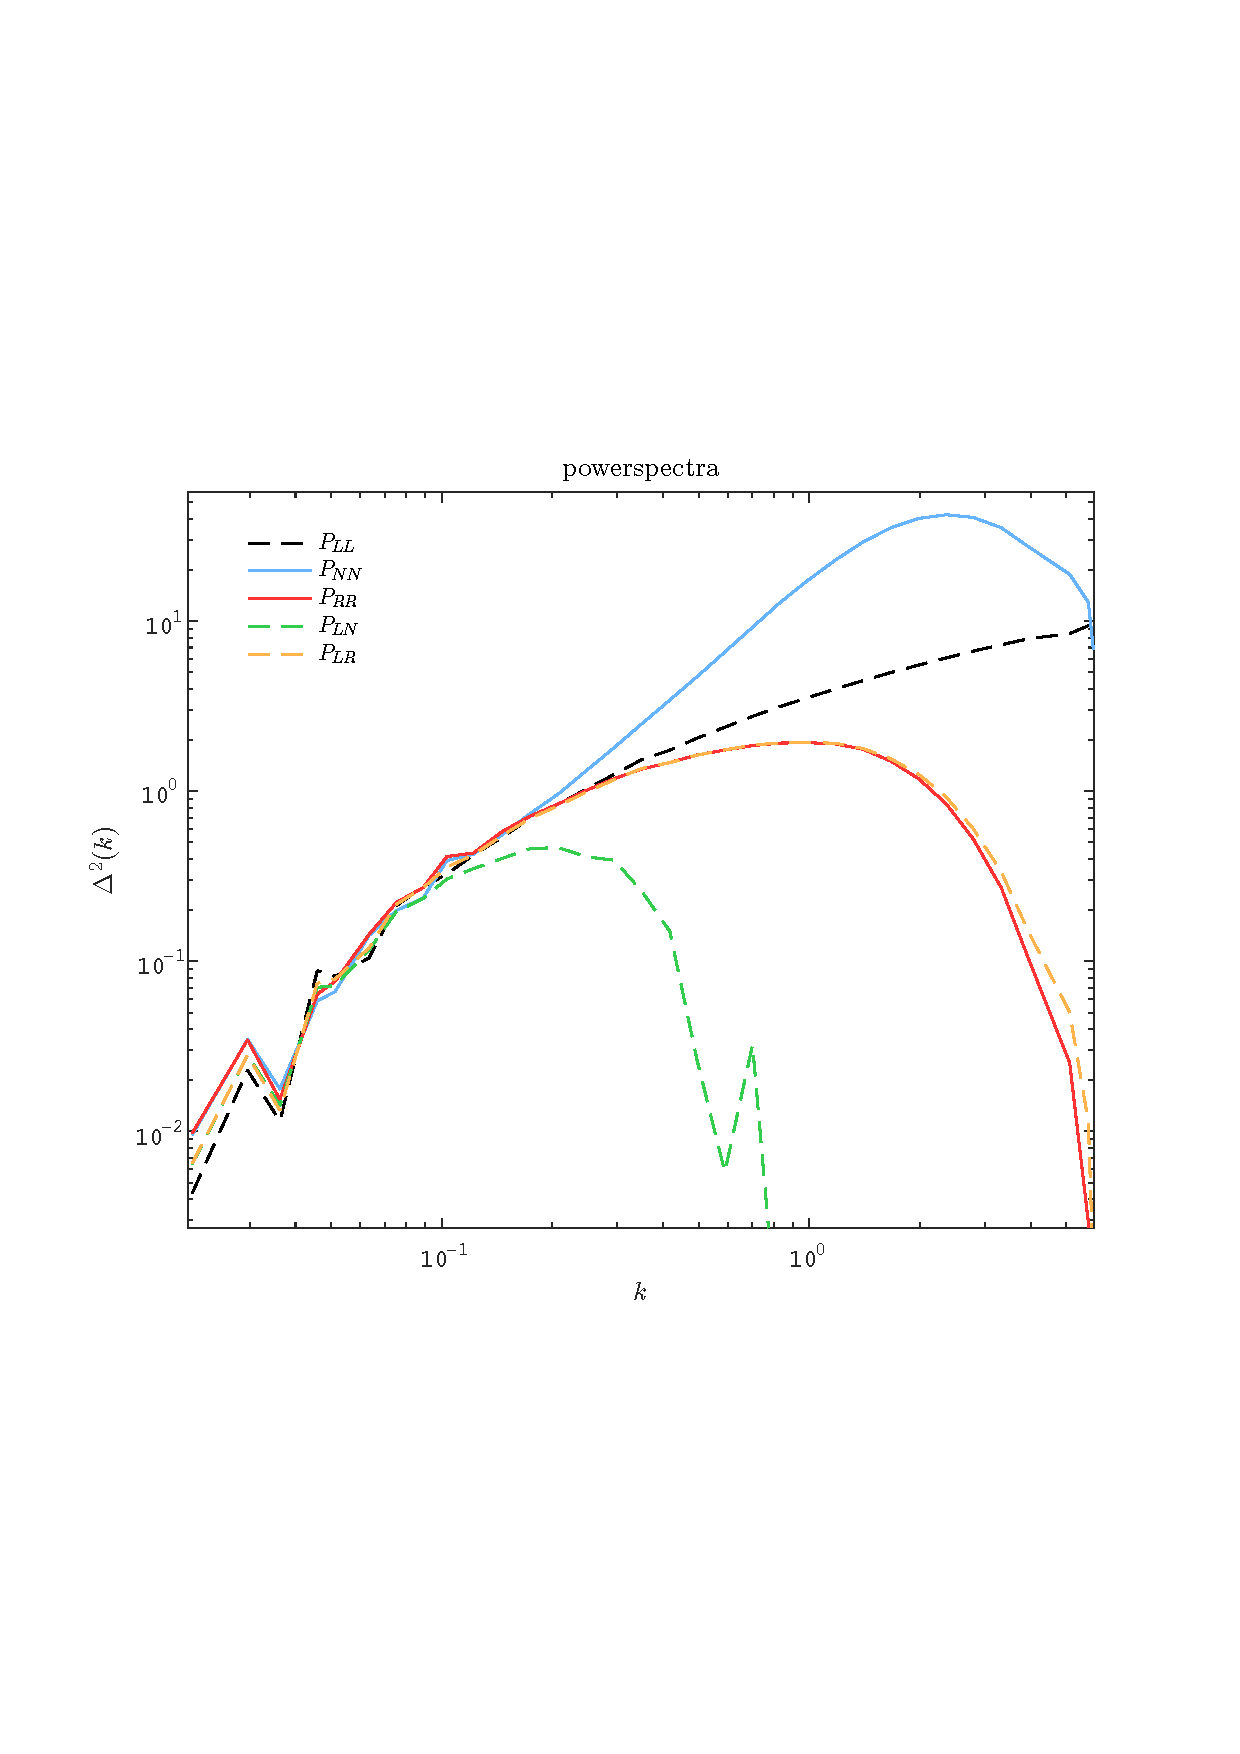
\includegraphics[width=1.0\linewidth]{fig1.pdf}
%  \caption{Caption goes here.}
%  \label{fig.1}
%\end{figure}

\section{Results}\label{sec.results}

Wiener filter.
Define
\begin{equation}
    r\equiv \frac{\left\langle\delta_L\delta_R\right\rangle}
    {\sqrt{\left\langle\delta_L\delta_L\right\rangle
    \left\langle\delta_R\delta_R\right\rangle}}
\end{equation}
and
\begin{equation}
    b^2\equiv \frac{\left\langle\delta_R\delta_R\right\rangle}
    {\left\langle\delta_L\delta_L\right\rangle}.
\end{equation}

We try to decompose $\delta_L$ into two components,
\begin{equation}\label{eq.decompose}
    \delta_L=r'\delta_R+\delta_N,
\end{equation}
where $r'\delta_R$ is completely correlated with $\delta_L$, and the uncorrelated part $\delta_N$ is generated by the nonlinear evolution. To do this, we first correlate equation (\ref{eq.decompose}) with $\delta_R$,
\begin{equation}\label{eq.correlate}
    \left\langle\delta_L\delta_R\right\rangle
    =r'\left\langle\delta_R\delta_R\right\rangle
    +\left\langle\delta_N\delta_R\right\rangle,
\end{equation}
and vanish the second term in the right-hand-side. Then
\begin{equation}
    r'=\frac{\left\langle\delta_L\delta_R\right\rangle}
    {\left\langle\delta_R\delta_R\right\rangle}=\frac{r}{b}.
\end{equation}
Then the mode-coupling term 
\begin{equation}
    \delta_N=\delta_L-\frac{r}{b}\delta_R.
\end{equation}
We next square equation (\ref{eq.decompose}) and gives
\begin{equation}\label{eq.square}
    \left\langle\delta_L\delta_L\right\rangle
    =\frac{r^2}{b^2}\left\langle\delta_R\delta_R\right\rangle
    +\left\langle\delta_N\delta_N\right\rangle
    +2\frac{r}{b}\left\langle\delta_R\delta_N\right\rangle,
\end{equation}
and the third term of right-hand-side also vanishes. As a result,
\begin{equation}
    \left\langle\delta_N\delta_N\right\rangle
    =\frac{1-r^2}{b^2}
    \left\langle\delta_R\delta_R\right\rangle
\end{equation}
and a Wiener filter can be constructed as
\begin{equation}
    W=\frac{r^2}{r^2+1-r^2}=r^2.
\end{equation}

From equation (\ref{eq.decompose}), multiplying $W$, we obtain the optimal reconstructed linear density field by
\begin{equation}
    \tilde\delta_L=W\frac{r}{b}\delta_R=\frac{r^3}{b}\delta_R.
\end{equation}
From equation (\ref{eq.square}), multiplying $W^2$, the reconstructed linear power spectrum is giving by
\begin{equation}
\begin{aligned}
    \tilde{P}&=W^2\left\langle\delta_L\delta_L\right\rangle  \\
    &=r^2\frac{r^2}{b^2}\left\langle\delta_R\delta_R\right\rangle +r^2\left\langle\delta_N\delta_N\right\rangle  \\
    &=\frac{r^2}{b^2}\left\langle\delta_R\delta_R\right\rangle.
\end{aligned}
\end{equation}




\section{Discussion and conclusion}\label{sec.discussion}
Discussion goes here.

\section*{Acknowledgements}
Acknowledgements goes here.

%\bibliographystyle{apsrev4-1}
\bibliographystyle{h-physrev3}
\bibliography{../haoran_ref}

\end{document}
